\section{The dance of the swans}
\label{sec:05-swans}

Several triangle centers were identified by Peter Moses which lie on the $X_9$-centered circumconic of any triangle. These are listed   in \cite[X(9)]{etc} as follows: $X_k$, $k=$88, 100, 162, 190, 651, 653, 655, 658, 660, 662, 673, 771, 799,  823, 897, 1156, 1492, 1821, 2349, 2580, 2581, 3257, 4598, 4599, 4604, 4606, 4607, 8052, 20332, 23707, 24624, 27834, 32680.

In \cite{reznik2020-ballet} we call such centers {\em swans}, since over billiard 3-periodics they will elegantly glide along the margins of an elliptic ``pond''.

The first four centers on said list are $X_k$, $k=$88, 100, 162, and 190, and are shown in \cref{fig:05-four-swans}.

\begin{figure}
    \centering
    \includegraphics[width=.7\textwidth]{pics_05_220_four_swans.png}
    \caption{A billiard 3-periodic (blue) and the swans $X_k$, $k=$88, 100, 162, and 190. \href{https://bit.ly/34vwQAt}{Live}. This \href{https://youtu.be/JdcJt5PExsw}{Video} shows 29 swans from Moses' list in \cite[X(9)]{etc}.}
    \label{fig:05-four-swans}
\end{figure}

Above we saw that the motion of $X_{100}$ is ``monotonic'' whereas that with $a/b>\alpha_{88}$ that of $X_{88}$ isn't. The next two swans in \cite{etc} are $X_{162}$ and $X_{190}$. 

\begin{proposition}
\label{prop:05-x162}
The motion of $X_{162}$ with respect to $P_1(t)$ is non-monotonic if $a/b>\alpha_{162}$ where $\alpha_{162}{\simeq}1.1639$ is the only positive root of:
\[ 5 x^8 + 3 x^6 - 32 x^4 + 52 x^2 - 36 \]
\end{proposition}

\begin{proof}
The trilinear coordinates of $X_{162}$ are given by
{\small 
\[  \frac {1}{ \left( s_2^{2}-  s_3^{2} \right)  \left( s_2^{2}+ s_3^{2}-
s_1^{2} \right) } :  \frac {1}{ \left( s_3^{2}-  s_1^{2} \right)  \left( s_3^{2}+ s_1^{2} -
s_2^{2} \right) }:\frac {1}{ \left( s_1^{2}-  s_2^{2} \right)  \left( s_1^{2}+ s_3^{2} -
s_3^{2}\right) }\cdot
\]
}

We use the standard parametrization for vertices of the confocal family found in \cref{sec:02-confocal-standard-param}. Using the trilinear coordinates above, we have   $X_{162}(t)=(x_{126}(t), y_{126}(t))$ 
  At $t=\frac{\pi}{2}$, $P_1=(0,b)$ and   $X_{162}(\frac{\pi}{2})= (0,b)$.
  
  Solve $x_{162}'(t)|_{t=\frac{\pi}{2}}=0$ for $a/b$. After some long algebraic symbolic manipulation, this is equivalent to solving $5 x^8 + 3 x^6 - 32 x^4 + 52 x^2 - 36=0$, whose positive roots is $  \alpha_{162} \simeq 1.16369.$
\end{proof}

Since $\alpha_{88}>\alpha_{162}$, setting $a/b>\alpha_{88}$ implies both centers will move non-monotonically. Curiously:

\begin{proposition}
With $a/b>1$, $X_{88}$ and $X_{162}$ never coincide. Therefore over the billiard 3-periodic family, they never cross each other.
\end{proposition}

\begin{proof}
Consider an elementary triangle $P_1=(-1,0)$, $P_2=(1,0)$ and $P_3=(u,v)$. Obtain cartesian coordinates for $X_{88}$ and $X_{162}$ using their trilinears. The equation $X_{88}=X_{162}$ is given by two algebraic equations $F(u,v,s_1,s_2)=G(u,v,s_1,s_2)=0$ of degree 17 with   $s_1=\sqrt{(u-1)^2+v^2}=\mid P_3-P_2\mid$ and $s_2=\sqrt{(u+1)^2+v^2}=\mid P_2-P_1\mid$.
Particular solutions of these equations are    equilateral triangles with $P_3=(0,\pm \sqrt{3})$ in which case $X_{88}$ and $X_{162}$ go to infinity, i.e., these centers can never meet with $a/b>1$.
%\textcolor{red}{sketch. A figura esta com %cores erradas. Vou corrigir mas nao consigo %agora pois o meu inkscape nao funciona mais %com a atualizacao do mac.}
\end{proof}

\begin{figure}
    \centering
    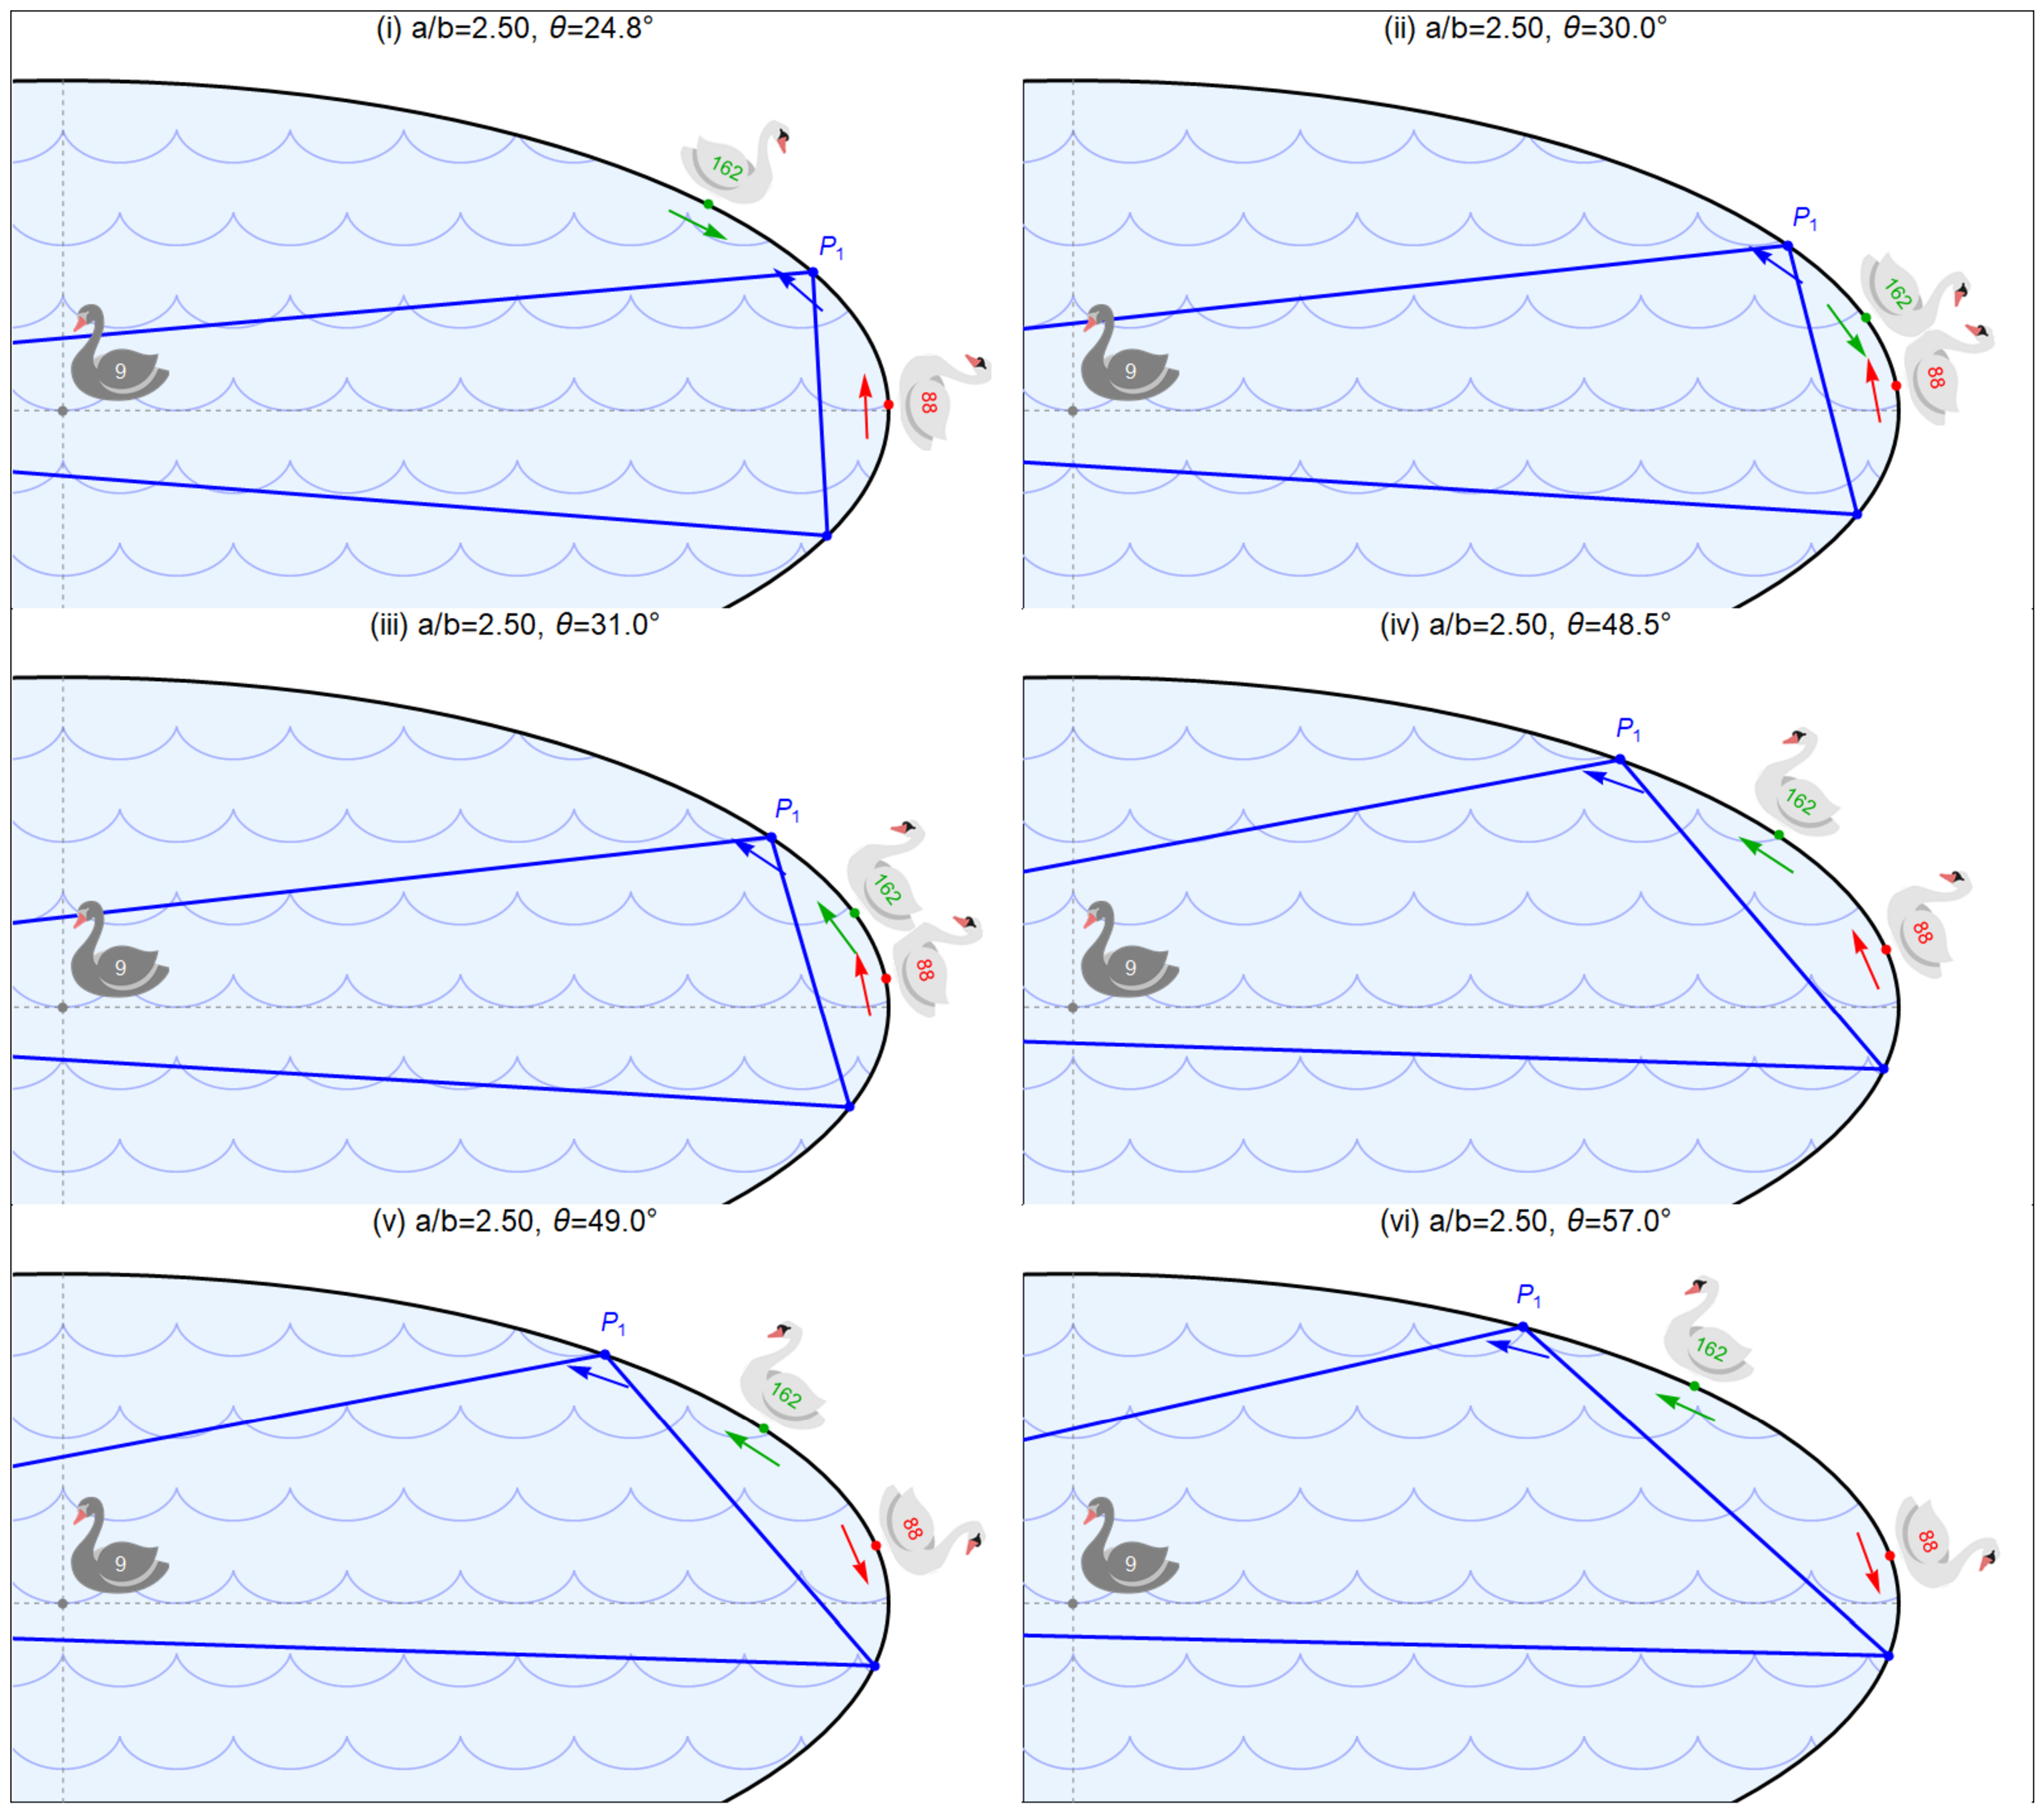
\includegraphics[width=\linewidth]{pics_05_200_swan_frames}
    \caption{The dance of swans $X_{88}$ and $X_{162}$ along the margins of an elliptic pond. (i) while $P_1$ moves CCW, $X_{88}$ and $X_{162}$ approach each other; (ii) at their closest, they almost kiss. (iii) Suddenly, $X_{162}$ reverses course, (iv) and a short-lived same-direction pursuit ensues. (v) An unswooned $X_{88}$ also changes course, (vi) with now both swimming away from each other. The duo meets again on 2nd, 3rd and 4th quadrants, where the dance steps are played back in alternating forward and backward order. A black mittenswan guards his clutch at the center of the lake. \href{https://youtu.be/ljGTtA1x-Sk}{Video}, two \href{https://bit.ly/3f6M9Wh}{Live} swans, four \href{https://bit.ly/3oDhMdd}{Live} swans.}
    \label{fig:x88-x162}
\end{figure}

The joint motion of $P_1(t)$, $X_{88}$, and $X_{162}$ can be visualized on the surface of a torus where the meridians (circles around the smaller radius) correspond to a given $t$ and the parallels represent a fixed location on the billiard boundary. As shown in \cref{fig:05-3d-torus}, the curves for $X_{88}$ and $X_{162}$ are thrice-winding, though never intersecting.

\begin{figure}
    \centering
    \includegraphics[width=\textwidth]{pics_05_210_torus_x88_x126_cropped}
    \caption{The coordinated motion of $P_1(t)$ (blue), $X_{88}$ (red) and $X_{162}$ (green) on the surface of a translucent torus, whose (i) meridians represent position along the elliptic billiard, and (ii) parallels the family parameter $t$. Notice the green and red curves are non-monotonic around the torus but never cross each other. A solid black meridian is wound at $t=0$ and a dashed one appears at one of the 12 instants of closest distance between $X_{88}$ and $X_{162}$, see \cref{que:05-x88-x162}.}
    \label{fig:05-3d-torus}
\end{figure}

Referring to \cref{fig:05-x190-angular-velocity}, we summarize the monotonicity in the motion of the first four swans on \cite{etc} with respect to a vertex of billiard 3-periodics as follows:

\begin{proposition}
\label{prop:05-x100-x190}
Over the family of billiard 3-periodics, for any $a/b>1$, the motion of $X_{100}$ and $X_{190}$ is monotonic and opposite with respect to that of a vertex in the family.
\end{proposition}

\begin{proposition}
\label{prop:05-x88-x162}
Over the family of billiard 3-periodics, if $a/b$ is below (resp. above) a certain $\alpha_{162}>1$ (resp. $\alpha_{88}>\alpha_{162}$), the motion of $X_{162}$ (resp. $X_{88}$) is monotonic and opposite (resp. non-monotonic) with respect to that of a vertex in the family. 
\end{proposition}

\begin{figure}
    \centering
    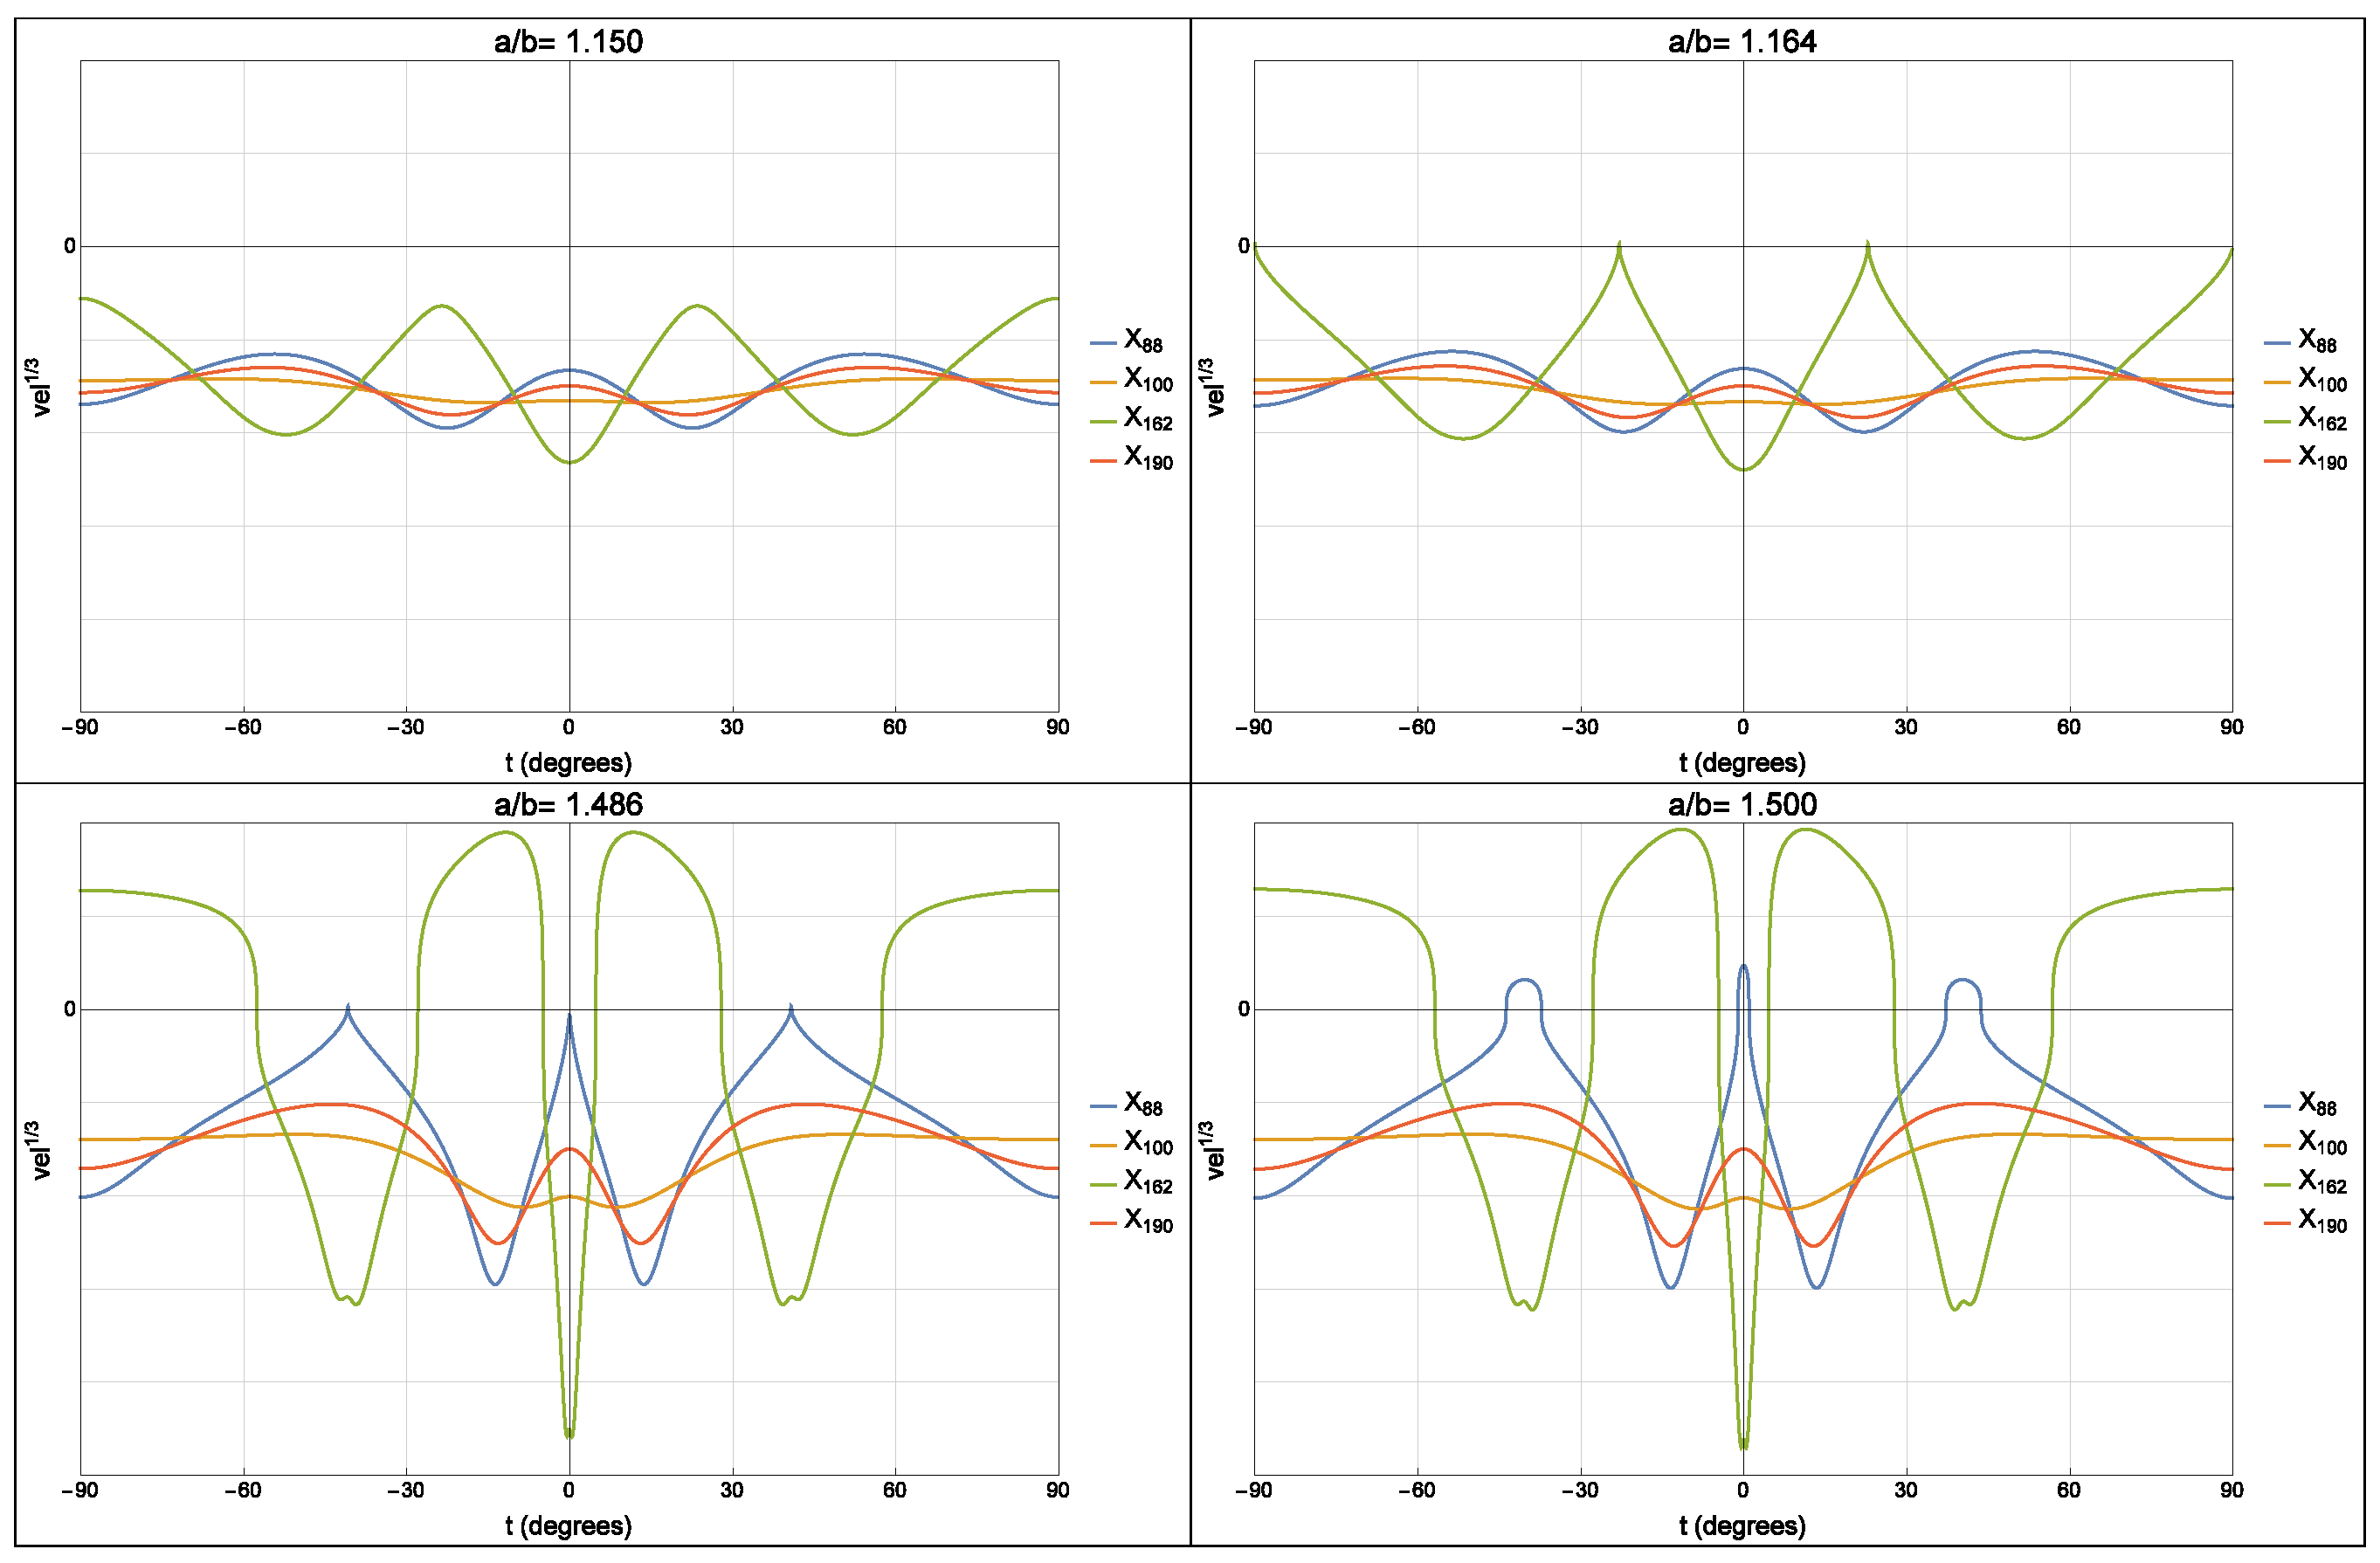
\includegraphics[width=\textwidth]{pics_05_230_xmany_vel.eps}
    \caption{Signed angular velocities of swans $X_k$, $k=$88,100,162,190 vs the parameter $t$ of $P_1(t)=[a\cos(t),b\sin(t)]$ of a billiard 3-periodic vertex, for various values of $a/b$. Cubic roots of the velocities are shown for better visualization near zero. \textbf{Top left:} $a/b=1.15$ is sufficiently small such that all centers move with variable, negative velocity (monotonic). \textbf{Top right:} At $a/b=\alpha_{162}{\geq}1.164$, the motion of $X_{162}$ comes to a stop at discrete values of $t$. \textbf{Bottom left:} At $a/b=\alpha_{88}{\geq}1.486$, it is $X_{88}$'s turn to touch zero velocity at discrete moments. \textbf{Bottom right:} at $a/b=1.5>\alpha_{88}>\alpha_{162}$, both $X_{162}$ and $X_{88}$ are engaged in non-monotonic motion. Notice $X_{100}$ and $X_{190}$ remain monotonic (negative velocity).}
    \label{fig:05-x190-angular-velocity}
\end{figure}
